% Provenance (never printed): see sources/outline_sources.md (Year 2: viscosity, density and
% volatiles of magmas; magma ascent; dykes, sills and plutons; contact aureoles).
% Curves from figdata/bachelor-2/magma.py (GRD 2008 viscosity, DensityX density, Moore 1998
% solubility data, erf sill cooling, Stefan solidification); exercise and problem values in
% the Book 4 scratch calculators calc/ch05.py and calc/ch05pb.py.
\chapter{Os magmas e seu alojamento}\label{ch:b2:magma-emplacement}

Um fundido basáltico a \qty{1200}{\celsius} escoa com uma viscosidade de cerca de
\qty{70}{Pa.s}: espesso, mas ele se derrama. Um fundido riolítico seco a \qty{800}{\celsius}
tem uma viscosidade perto de \qty{e11}{Pa.s}, e um bloco dele levaria horas para ceder
visivelmente sob o próprio peso. Entre os dois há dez ordens de grandeza, mais
do que entre a água e o basalto, e a maior parte da diferença vem de duas
coisas: a sílica, que liga o fundido em uma rede, e a temperatura,
várias centenas de graus mais baixa nos \omterm{def:b2:magma-emplacement:magma}{magmas} silícicos. Alguns por cento de
água dissolvida, que um \omterm{def:b2:magma-emplacement:magma}{magma} riolítico pode conter em profundidade, reduzem sua viscosidade
por um fator \num{e5}, e esse efeito se perde de novo quando o \omterm{def:b2:magma-emplacement:magma}{magma} sobe e a
água sai na forma de bolhas. Esses números decidem se um \omterm{def:b2:magma-emplacement:magma}{magma} chega à
superfície tranquilamente, explode ou se solidifica a quilômetros de profundidade como um \omterm{def:b2:magma-emplacement:bodies}{dique}, uma \omterm{def:b2:magma-emplacement:bodies}{soleira} ou um
\omterm{def:b2:magma-emplacement:bodies}{plúton}. Este capítulo trata um \omterm{def:b2:magma-emplacement:magma}{magma} como um material: sua densidade, sua viscosidade e seus
voláteis, a física de sua ascensão por fraturas e como corpos isolados, as formas que ele
assume quando para, e o calor que cede às rochas ao seu redor.
% ledger: grd08:model, grd08:range, moore98:melts

\begin{recall}
\textbf{Escoamento viscoso} (livros de física, volume do segundo ano): em um fluido newtoniano de
viscosidade $\eta$, a tensão de cisalhamento é $\eta$ vezes o gradiente de velocidade; entre
duas paredes paralelas, um gradiente de pressão impõe um perfil parabólico (de Poiseuille
plano); uma esfera que se move lentamente em um fluido viscoso sofre o arrasto de Stokes
$6\pi\eta a v$. \textbf{Condução de calor} (mesmo volume): a temperatura obedece a
$\partial T/\partial t = \kappa\,\partial^2T/\partial x^2$, com difusividade $\kappa = k/(\rho
c)$, e um degrau de temperatura se espalha como uma função erro sobre uma distância da
ordem de $\sqrt{\kappa t}$. \textbf{Empuxo} (livros de física, volume do primeiro ano): um corpo
imerso em um fluido mais denso sofre uma força resultante para cima igual ao peso do fluido
deslocado menos o seu próprio. \textbf{Equilíbrio químico} (livros de química): no
equilíbrio, as atividades dos produtos e dos reagentes satisfazem a lei de ação
das massas com uma constante $K$ que depende da temperatura. Do volume do primeiro ano
desta série: a pressão litostática $p = \rho g z$ e a geoterma; dos
volumes escolares: rochas máficas e félsicas, fenocristais e texturas porfiríticas.
\end{recall}

\section{O que é um magma}

\begin{definition}[Magma]\label{def:b2:magma-emplacement:magma}
Um \emph{magma}\index{magma} é rocha fundida ou parcialmente fundida sob a superfície: um
\emph{fundido silicático}\index{fundido silicático}, o líquido formado sobretudo de silício,
oxigênio e cátions metálicos, junto com os cristais e as bolhas de gás que ele carrega.
Um \emph{mush cristalino}\index{mush cristalino} é um magma tão rico em cristais que estes
se tocam e formam um arcabouço: ele não pode escoar como um líquido, e seu fundido só pode
se mover pelos poros entre os cristais.
\end{definition}

A composição do fundido é dada, como para as rochas, em porcentagem em peso de
óxidos. Três fundidos servem de referência ao longo do capítulo, todos eles
estudados em laboratório: um basalto toleítico dragado em uma dorsal meso-oceânica
(cerca de \qty{51}{\percent} de SiO$_2$, \qty{12}{\percent} de óxido de ferro, \qty{7}{\percent}
de MgO), um andesito (\qty{63}{\percent} de SiO$_2$) e um riolito (\qty{78}{\percent} de
SiO$_2$, \qty{8}{\percent} de Na$_2$O $+$ K$_2$O e quase nada de ferro ou de magnésio).
Suas temperaturas de erupção diferem tanto quanto suas composições: os \omterm{def:b2:magma-emplacement:magma}{magmas} basálticos
entram em erupção a \qtyrange{1000}{1200}{\celsius} (a lava que corre em um tubo no
Kilauea foi medida perto de \qty{1200}{\celsius}), os \omterm{def:b2:magma-emplacement:magma}{magmas} andesíticos a
\qtyrange{800}{1000}{\celsius}, os \omterm{def:b2:magma-emplacement:magma}{magmas} riolíticos a \qtyrange{650}{800}{\celsius}.
Um \omterm{def:b2:magma-emplacement:magma}{magma} riolítico é mais frio porque é o resíduo de uma longa cristalização
ou o primeiro fundido de rochas crustais, dois processos que ocorrem a baixa temperatura
(\cref{ch:b2:magmatic-differentiation}).
% ledger: moore98:melts, tulane:magma-types, earle:kilauea-lava

O teor de cristais decide se um \omterm{def:b2:magma-emplacement:magma}{magma} escoa. Estudos de campo e geocronológicos
de grandes corpos graníticos concluem que o escoamento magmático em massa exige uma fração
de fundido de pelo menos \qtyrange{30}{50}{\percent} em volume; abaixo disso, os
cristais estão soldados aos seus vizinhos e o material se deforma como um sólido com
poros cheios de fundido. Pensa-se que boa parte do \omterm{def:b2:magma-emplacement:magma}{magma} armazenado na crosta esteja
nesse estado, como um mush que volta a ficar móvel quando \omterm{def:b2:magma-emplacement:magma}{magma} quente é acrescentado por
baixo.
% ledger: glazner04:tuolumne

\section{Densidade e viscosidade}

\subsection{A densidade de um fundido}

Um \omterm{def:b2:magma-emplacement:magma}{fundido silicático} não tem rede cristalina, mas seu volume ainda pode ser construído a partir
de seus componentes. Experimentos com muitos fundidos mostram que cada óxido contribui com um
volume quase fixo por mol, seu volume molar parcial, que varia lenta e
linearmente com a temperatura e a pressão; o volume do fundido é a soma
dessas contribuições. A tabela abaixo dá os valores usados neste capítulo.

\begin{table}[ht]
\centering\small
\begin{tabular}{lrrr}
\hline
Óxido & $\bar V_i$ (\unit{cm^3/mol}) & $\partial\bar V_i/\partial T$ (\num{e-3}\,\unit{cm^3/(mol.K)}) & $\partial\bar V_i/\partial p$ (\num{e-4}\,\unit{cm^3/(mol.bar)}) \\
\hline
SiO$_2$  & 26.86 & 0     & $-1.89$ \\
Al$_2$O$_3$ & 37.42 & 2.62 & $-2.26$ \\
FeO      & 12.68 & 3.69  & $-0.45$ \\
MgO      & 12.02 & 3.27  & $0.27$ \\
CaO      & 16.90 & 3.74  & $0.34$ \\
Na$_2$O  & 29.65 & 7.68  & $-2.40$ \\
K$_2$O   & 47.28 & 12.08 & $-6.75$ \\
H$_2$O   & 22.9  & 9.5   & $-3.20$ \\
\hline
\end{tabular}
\caption{Volumes molares parciais dos componentes óxidos nos \omterm{def:b2:magma-emplacement:magma}{fundidos silicáticos} a
\qty{1}{bar}, com suas derivadas em relação à temperatura e à pressão. Temperatura
de referência \qty{1773}{K} (FeO \qty{1723}{K}, H$_2$O \qty{1273}{K}). Dados:
compilação do programa DensityX (Iacovino e Till, 2019).}
\label{tab:b2:magma-emplacement:volumes}
\end{table}
% ledger: densityx:volumes

\begin{proposition}[Densidade de um fundido silicático]\label{prop:b2:magma-emplacement:density}
Suponha-se que um fundido contenha componentes óxidos $i$ de frações molares $X_i$, massas molares
$M_i$ e volumes molares parciais $\bar V_i(T, p) = \bar V_i^{\circ} + (\partial\bar
V_i/\partial T)(T - T_{\mathrm{ref}}) + (\partial\bar V_i/\partial p)(p - p_{\mathrm{ref}})$.
Se os componentes se misturam idealmente em volume,
\[
\rho = \frac{\sum_i X_i M_i}{\sum_i X_i \bar V_i(T,p)}.
\]
\end{proposition}

\begin{proof}
Um mol de fundido contém $X_i$ mols do componente $i$, de massa $X_iM_i$. A mistura
ideal em volume significa que cada mol do componente $i$ acrescenta o volume $\bar V_i$
quaisquer que sejam os outros, de modo que o mol de fundido ocupa $\sum_i X_i\bar V_i$. A
densidade é a razão entre os dois.
\end{proof}

A água tem uma massa molar de apenas \qty{18}{g/mol}, mas um volume molar parcial de
\qty{22.9}{cm^3/mol}, próximo do da sílica: ela reduz fortemente a densidade de um
fundido. Aplicada aos três fundidos de referência, a proposição dá
\qty{2730}{kg/m^3} para o basalto a \qty{1200}{\celsius}, \qty{2480}{kg/m^3} para
o andesito a \qty{1000}{\celsius} e \qty{2340}{kg/m^3} para o riolito seco
a \qty{850}{\celsius}; um por cento de água dissolvida tira cerca de
\qty{70}{kg/m^3} do basalto, tanto quanto várias centenas de graus de aquecimento.
Um fundido basáltico é portanto mais leve que o peridotito mantélico de onde vem
(cerca de \qty{3380}{kg/m^3} sob a crosta no modelo de Terra de referência) e um
pouco mais leve que a crosta inferior desse modelo (\qty{2900}{kg/m^3}), ao passo que um
fundido riolítico é mais leve até que sua crosta superior (\qty{2600}{kg/m^3}). Essa diferença impele os \omterm{def:b2:magma-emplacement:magma}{magmas}
para cima.
% ledger: densityx:volumes, densityx:water, data:prem

\subsection{A viscosidade}

A viscosidade de um \omterm{def:b2:magma-emplacement:magma}{fundido silicático} é fixada pela rede de tetraedros SiO$_4$
ligados por oxigênios compartilhados: para escoar, o fundido precisa romper e refazer
ligações silício--oxigênio. A sílica e a alumina constroem a rede; os cátions de
magnésio, de ferro, de cálcio e os álcalis a rompem, e a água também, que
transforma oxigênios em ponte em grupos hidroxila. As medidas de laboratório em fundidos
naturais cobrem mais de quinze ordens de grandeza, de \qty{0.1}{Pa.s} a
\qty{e14}{Pa.s}, e não seguem uma lei de Arrhenius simples: a viscosidade
cresce mais depressa que uma exponencial em $1/T$ à medida que o fundido se resfria em direção à sua transição
vítrea.
% ledger: grd08:range

\begin{proposition}[Lei de Vogel--Fulcher--Tammann]\label{prop:b2:magma-emplacement:vft}
A viscosidade de um \omterm{def:b2:magma-emplacement:magma}{fundido silicático} de composição fixa segue, a alguns
décimos de unidade logarítmica,
\[
\log_{10}\eta = A + \frac{B}{T - C},
\]
com $\eta$ em pascal-segundos e $T$ em kelvins. Para os fundidos naturais, $A$ é próximo
de $-4.55$ qualquer que seja a composição; $B$ e $C$ (em kelvins) são combinações
lineares das porcentagens molares dos óxidos, com alguns produtos entre elas,
ajustadas a cerca de \num{1800} medidas.
\end{proposition}
\admitted
% ledger: grd08:model, grd08:range

A figura abaixo mostra a lei para os três fundidos de referência e para o
riolito com água dissolvida. A \qty{1200}{\celsius} o basalto tem
$\eta \approx \qty{70}{Pa.s}$; o andesito a \qty{1000}{\celsius}, cerca de
\qty{e6}{Pa.s}; o riolito seco a \qty{800}{\celsius}, cerca de $10^{10.9}$\,\unit{Pa.s}.
Quatro por cento de água levam o mesmo riolito a $10^{5.5}$\,\unit{Pa.s}, seis
por cento a $10^{4.6}$\,\unit{Pa.s}. Uma equação independente, ajustada apenas a fundidos
graníticos hidratados, dá os mesmos valores a meia unidade logarítmica
(\cref{exo:b2:magma-emplacement:1}). O efeito da água é máximo a baixa temperatura, onde alguns
décimos de por cento alteram a viscosidade em ordens de grandeza.
% ledger: grd08:model, hd96:model, moore98:melts

\begin{omfigure}
\centering
\begin{tikzpicture}
\begin{axis}[omrecord, width=0.86\linewidth, height=6.4cm,
  xmin=600, xmax=1400, ymin=0, ymax=15,
  xlabel={temperatura (\unit{\celsius})}, ylabel={$\log_{10}\eta$ (\unit{Pa.s})},
  legend pos=north east, legend style={font=\scriptsize},
  tick label style={font=\scriptsize}, label style={font=\small}]
\addplot[very thick, black, restrict x to domain=1000:1400] table[x=T_C, y=basalt] {figdata/out/bachelor-2-magma-visc.dat};
\addlegendentry{basalto, seco}
\addplot[very thick, brown, restrict x to domain=800:1300] table[x=T_C, y=andesite] {figdata/out/bachelor-2-magma-visc.dat};
\addlegendentry{andesito, seco}
\addplot[very thick, red!70!black, restrict x to domain=650:1100] table[x=T_C, y=rhyolite] {figdata/out/bachelor-2-magma-visc.dat};
\addlegendentry{riolito, seco}
\addplot[thick, red!70!black, dashed, restrict x to domain=650:1000] table[x=T_C, y=rhy2] {figdata/out/bachelor-2-magma-visc.dat};
\addlegendentry{riolito, 2 \% H$_2$O}
\addplot[thick, red!70!black, densely dotted, restrict x to domain=650:1000] table[x=T_C, y=rhy4] {figdata/out/bachelor-2-magma-visc.dat};
\addlegendentry{riolito, 4 \% H$_2$O}
\addplot[thick, red!70!black, dashdotted, restrict x to domain=650:1000] table[x=T_C, y=rhy6] {figdata/out/bachelor-2-magma-visc.dat};
\addlegendentry{riolito, 6 \% H$_2$O}
\end{axis}
\end{tikzpicture}
\par\smallskip{\small Viscosidade dos \omterm{def:b2:magma-emplacement:magma}{fundidos silicáticos} em função da temperatura, pela
lei de Vogel--Fulcher--Tammann com os parâmetros dependentes da composição de
Giordano, Russell e Dingwell (2008). Basalto: um toleíto de dorsal meso-oceânica;
andesito e riolito: fundidos de referência de laboratório (Moore e colaboradores, 1998). Cada
curva é traçada no intervalo de temperaturas em que tal \omterm{def:b2:magma-emplacement:magma}{magma} pode estar fundido.}
\end{omfigure}
% ledger: grd08:model, moore98:melts

Os cristais tornam um \omterm{def:b2:magma-emplacement:magma}{magma} ainda mais rígido. Uma suspensão de partículas rígidas resiste
ao cisalhamento mais que seu líquido sozinho, porque o líquido precisa contornar as
partículas, e, quando as partículas estão apertadas a ponto de se tocar, elas se travam em um
arcabouço.

\begin{proposition}[Relação de Einstein--Roscoe]\label{prop:b2:magma-emplacement:roscoe}
Uma suspensão de uma fração volumétrica $\phi$ de esferas rígidas em um líquido newtoniano
de viscosidade $\eta_{\ell}$ tem a viscosidade
\[
\eta = \eta_{\ell}\,(1 - R\phi)^{-2.5}, \qquad R = 1/\phi_m \approx 1.35,
\]
onde $\phi_m$ é a fração de empacotamento máximo, na qual a suspensão trava. Para
$\phi$ pequeno, isso se reduz à relação de Einstein, $\eta = \eta_{\ell}(1 + 2.5\phi)$.
\end{proposition}
\admitted
% ledger: kolz22:einstein-roscoe

Vinte por cento de cristais dobram a viscosidade, quarenta por cento a multiplicam por
sete, sessenta por cento por mais de sessenta (\cref{exo:b2:magma-emplacement:5}); nos \omterm{def:b2:magma-emplacement:magma}{magmas} reais, onde os
cristais são alongados e de muitos tamanhos, o travamento chega antes, perto dos
\qtyrange{50}{70}{\percent} de cristais nos quais as evidências de campo situam o
fim do escoamento em massa.

\section{Os voláteis}

\begin{definition}[Voláteis magmáticos]\label{def:b2:magma-emplacement:volatiles}
Um \emph{volátil magmático}\index{volátil magmático} é um componente de um \omterm{def:b2:magma-emplacement:magma}{magma} que
está dissolvido no fundido em profundidade e forma uma fase gasosa separada a baixa
pressão: principalmente a água, depois o dióxido de carbono, depois as espécies de enxofre. A \emph{exsolução
de voláteis}\index{exsolução de voláteis} é a separação de um volátil do
fundido em bolhas de gás. A \emph{pressão de saturação
em voláteis}\index{pressão de saturação em voláteis} de um fundido é a pressão abaixo da qual
seus voláteis dissolvidos excedem sua solubilidade, de modo que uma fase gasosa precisa se formar.
\end{definition}

Os \omterm{def:b2:magma-emplacement:magma}{magmas} máficos carregam tipicamente \qtyrange{1}{3}{\percent} de voláteis em massa,
os \omterm{def:b2:magma-emplacement:magma}{magmas} intermediários \qtyrange{3}{4}{\percent}, os \omterm{def:b2:magma-emplacement:magma}{magmas} félsicos
\qtyrange{4}{7}{\percent}, e a exsolução de \qtyrange{4}{6}{\percent} de
água impele a maioria das erupções explosivas. A quantidade de água que um fundido pode conter depende
sobretudo da pressão. A figura abaixo mostra medidas em fundidos basálticos e
riolíticos mantidos sob uma pressão de água conhecida até a saturação, depois temperados
em vidro e analisados: a solubilidade cresce rapidamente a baixa pressão e mais
lentamente a alta pressão.
% ledger: earle:volatiles, moore98:arc-water, moore98:h2o

\begin{proposition}[Lei da raiz quadrada para a água]\label{prop:b2:magma-emplacement:sqrt}
Suponha-se que a água se dissolva em um \omterm{def:b2:magma-emplacement:magma}{fundido silicático} sobretudo como grupos hidroxila, pela
reação $\mathrm{H_2O\,(\text{gás})} + \mathrm{O^{2-}\,(fundido)} \rightleftharpoons
2\,\mathrm{OH^-\,(fundido)}$, com o oxigênio do fundido em grande excesso. Então, a
baixos teores de água, a água dissolvida é proporcional à raiz quadrada da
pressão de água: $w \approx s\sqrt{p}$, sendo $s$ uma constante do fundido e da
temperatura.
\end{proposition}

\begin{proof}
A lei de ação das massas dá $x_{\mathrm{OH}}^2 = K\,x_{\mathrm{O}}\,f$, onde $f$ é
a fugacidade da água (próxima de sua pressão a pressões moderadas) e os $x$
são frações molares. O oxigênio do fundido está em grande excesso, de modo que
$x_{\mathrm{O}}$ permanece quase constante, e $x_{\mathrm{OH}} = \sqrt{Kx_{\mathrm{O}}}\,
\sqrt f$. Cada molécula de água dissolvida produz duas hidroxilas, de modo que a água
dissolvida é $x_{\mathrm{OH}}/2$, proporcional a $\sqrt f$. A teores mais altos, parte
da água se dissolve como moléculas, em proporção ao próprio $f$, e a
solubilidade cresce mais depressa que a raiz quadrada (\cref{exo:b2:magma-emplacement:10}).
\end{proof}

Ajustada por mínimos quadrados às medidas, $w = s\sqrt p$ dá
$s = 0.34$ por cento em peso por $\sqrt{\unit{MPa}}$ para os basaltos e
$s = 0.44$ para os riolitos; toda medida fica a menos de um por cento de
água de sua curva. A pressão de saturação de um fundido com $w$ por cento
de água é então $p_s = (w/s)^2$: \qty{129}{MPa} para um riolito com
\qty{5}{\percent} de água, cerca de \qty{5}{km} de profundidade na crosta, mas apenas
\qty{2}{MPa} para um basalto com \qty{0.5}{\percent}, cem metros ou menos.
% ledger: moore98:h2o

\begin{omfigure}
\centering
\begin{tikzpicture}
\begin{axis}[omrecord, width=0.8\linewidth, height=6cm,
  xmin=0, xmax=300, ymin=0, ymax=9,
  xlabel={pressão de água (\unit{MPa})}, ylabel={H$_2$O dissolvida (\% em peso)},
  legend pos=south east, legend style={font=\scriptsize},
  tick label style={font=\scriptsize}, label style={font=\small}]
\addplot[very thick, red!70!black] table[x=P_MPa, y=rhyolite] {figdata/out/bachelor-2-magma-solub-fit.dat};
\addlegendentry{riolito, $0.44\sqrt p$}
\addplot[only marks, mark=*, mark size=2pt, red!70!black] table[x=P_MPa, y=w] {figdata/out/bachelor-2-magma-solub-rhyolite-data.dat};
\addlegendentry{riolito, medidas}
\addplot[very thick, black] table[x=P_MPa, y=basalt] {figdata/out/bachelor-2-magma-solub-fit.dat};
\addlegendentry{basalto, $0.34\sqrt p$}
\addplot[only marks, mark=square*, mark size=2pt, black] table[x=P_MPa, y=w] {figdata/out/bachelor-2-magma-solub-basalt-data.dat};
\addlegendentry{basalto, medidas}
\end{axis}
\end{tikzpicture}
\par\smallskip{\small Solubilidade da água em fundidos basálticos e riolíticos a
\qtyrange{800}{1200}{\celsius} em função da pressão de água: medidas compiladas
por Moore e colaboradores (1998), e leis de raiz quadrada ajustadas por mínimos quadrados. A
\qty{100}{MPa}, cerca de \qty{4}{km} de profundidade na crosta, um riolito pode conter
\qty{4.4}{\percent} de água, um basalto \qty{3.4}{\percent}.}
\end{omfigure}
% ledger: moore98:h2o

O dióxido de carbono é muito menos solúvel que a água. Ele se dissolve como moléculas nos
riolitos e como grupos carbonato nos basaltos, mais nos fundidos alcalinos que nos
toleítos, e sua solubilidade também cresce com a pressão. Um \omterm{def:b2:magma-emplacement:magma}{magma} que carrega os dois
gases começa portanto a exsolver em profundidade, com um gás muito rico em CO$_2$, e o
gás se enriquece em água à medida que o \omterm{def:b2:magma-emplacement:magma}{magma} sobe. Os basaltos emitidos no fundo
do mar profundo contêm vesículas com mais de \qty{95}{\percent} de CO$_2$, o que exigiu
saturação em CO$_2$ mesmo sob \qty{5}{km} de água. As estimativas do teor inicial
de CO$_2$ dos basaltos parentais do Kilauea vão de \qtyrange{0.2}{0.6}{\percent},
e inclusões de fundido aprisionadas em seus cristais de olivina registram pressões de saturação
de até \qty{500}{MPa}.
% ledger: lowenstern01:co2, lowenstern01:basalts

O gás exsolvido ocupa um grande volume. Um por cento de água em um \omterm{def:b2:magma-emplacement:magma}{magma} a
\qty{900}{\celsius} ocupa, como gás ideal, cerca de \qty{12}{\percent} do
volume a \qty{100}{MPa}, \qty{57}{\percent} a \qty{10}{MPa} e mais de
\qty{99}{\percent} à pressão atmosférica (\cref{exo:b2:magma-emplacement:7}). As bolhas reduzem ainda mais a
densidade do \omterm{def:b2:magma-emplacement:magma}{magma} e o impelem para cima mais depressa; em um \omterm{def:b2:magma-emplacement:magma}{magma} viscoso
elas não conseguem escapar, e o \cref{ch:b2:eruptive-styles} mostra como elas o fragmentam.

\section{A ascensão}

Um corpo de \omterm{def:b2:magma-emplacement:magma}{magma} menos denso que suas encaixantes sofre uma força de empuxo de
$\Delta\rho\,g$ por unidade de volume, onde $\Delta\rho$ é a diferença de densidade. Ele
pode subir de duas maneiras: por uma fratura que abre à sua frente, ou como um corpo quente e
mole que empurra a rocha ao redor para os lados.

\subsection{Os diques}

Em profundidade a rocha está sob uma grande pressão litostática, mas uma fratura preenchida
por \omterm{def:b2:magma-emplacement:magma}{magma} a uma pressão ligeiramente superior à tensão principal mínima pode
se abrir e se alongar em sua ponta. O \omterm{def:b2:magma-emplacement:magma}{magma} preenche a fratura à medida que ela cresce, e o resultado
é uma fina lâmina de \omterm{def:b2:magma-emplacement:magma}{magma}, com metros de largura e quilômetros de comprimento, que abre caminho
para cima: um \omterm{def:b2:magma-emplacement:bodies}{dique} em formação. O \omterm{def:b2:magma-emplacement:magma}{magma} escoa então entre duas paredes quase
paralelas.

\begin{proposition}[Escoamento do magma em um dique]\label{prop:b2:magma-emplacement:poiseuille}
Um \omterm{def:b2:magma-emplacement:magma}{magma} newtoniano de viscosidade $\eta$, impelido para cima por um gradiente de pressão $G$
(para um escoamento por empuxo, $G = \Delta\rho\,g$) entre duas paredes paralelas separadas por uma distância $w$,
escoa com a velocidade média
\[
\bar u = \frac{G w^2}{12\,\eta},
\]
e o fluxo volumétrico por unidade de comprimento de \omterm{def:b2:magma-emplacement:bodies}{dique} é $q = \bar u w = G w^3/(12\eta)$.
\end{proposition}

\begin{proof}
Em escoamento laminar estacionário, o perfil de velocidade através do \omterm{def:b2:magma-emplacement:bodies}{dique} é a parábola
de Poiseuille plana $u(x) = \frac{G}{2\eta}\left(\frac{w^2}{4} - x^2\right)$, para
$-w/2 \le x \le w/2$, que se anula nas duas paredes. Sua média é
$\bar u = \frac1w\int_{-w/2}^{w/2}u\,dx = \frac{G}{2\eta}\left(\frac{w^2}{4} -
\frac{w^2}{12}\right) = \frac{Gw^2}{12\eta}$.
\end{proof}

O cubo da largura torna os \omterm{def:b2:magma-emplacement:bodies}{diques} largos muito mais eficientes que os estreitos. Um
basalto de \qty{100}{Pa.s} em um \omterm{def:b2:magma-emplacement:bodies}{dique} de \qty{1}{m} de largura, com $\Delta\rho =
\qty{300}{kg/m^3}$, sobe a cerca de \qty{2.5}{m/s} e atravessa \qty{10}{km} de
crosta em uma hora; um riolito de \qty{e6}{Pa.s} no mesmo \omterm{def:b2:magma-emplacement:bodies}{dique} levaria mais
de um ano, e se solidificaria no caminho, de modo que os \omterm{def:b2:magma-emplacement:magma}{magmas} silícicos precisam de \omterm{def:b2:magma-emplacement:bodies}{diques} muito mais
largos (\cref{exo:b2:magma-emplacement:6}). O número de Reynolds $\rho\bar u w/\eta$ desses escoamentos
é pequeno o bastante para que permaneçam laminares. As velocidades de ascensão estimadas para os \omterm{def:b2:magma-emplacement:magma}{magmas}
durante as erupções separam as erupções efusivas, abaixo de cerca de \qty{0.1}{m/s}, das
explosivas, acima disso, com um intervalo de transição de \qtyrange{0.005}{0.25}{m/s}
em que os dois estilos ocorrem; os kimberlitos, que vêm de
profundidades além de \qty{150}{km}, foram estimados em \qtyrange{0.1}{30}{m/s}, e
um estudo de difusão de um deles dá \qtyrange{0.02}{0.23}{m/s} em média sobre
os últimos \qtyrange{80}{110}{km}, uma viagem de \numrange{5}{74} dias.
% ledger: cassidy18:ascent, casetta23:kimberlite

\subsection{Os diápiros}

\begin{definition}[Diápiro, nível de flutuabilidade neutra, desmoronamento magmático]\label{def:b2:magma-emplacement:ascent}
Um \emph{diápiro}\index{diápiro} é um corpo de material flutuante, \omterm{def:b2:magma-emplacement:magma}{magma} ou rocha parcialmente
fundida, que sobe através de suas encaixantes fazendo-as escoar para os lados. O
\emph{nível de flutuabilidade neutra}\index{nível de flutuabilidade neutra} de um \omterm{def:b2:magma-emplacement:magma}{magma} é a
profundidade na qual sua densidade é igual à da rocha ao redor: abaixo dele o
\omterm{def:b2:magma-emplacement:magma}{magma} flutua, acima dele é mais denso que suas encaixantes. O \emph{desmoronamento
magmático}\index{desmoronamento magmático} é o desprendimento de blocos da rocha das paredes ou do
teto, que afundam no \omterm{def:b2:magma-emplacement:magma}{magma}; os blocos que ficam inclusos na rocha solidificada
são xenólitos.
\end{definition}
% ledger: earle:intrusive-bodies

\begin{proposition}[Ascensão de Stokes]\label{prop:b2:magma-emplacement:stokes}
Uma esfera de raio $a$ e déficit de densidade $\Delta\rho$ que sobe lentamente através de um
meio newtoniano de viscosidade $\eta$ atinge a velocidade terminal
\[
v = \frac{2\,\Delta\rho\,g\,a^2}{9\,\eta}
\]
se for rígida, e $1.5$ vez essa velocidade se for um fluido de viscosidade desprezível.
\end{proposition}
\admitted

A rocha em torno de um \omterm{def:b2:magma-emplacement:ascent}{diápiro} não é um fluido de \qty{100}{Pa.s}, mas um sólido quente,
cuja viscosidade é muitas ordens de grandeza maior que a de qualquer fundido: na
crosta, uma esfera de \omterm{def:b2:magma-emplacement:magma}{magma} de um quilômetro de diâmetro sobe apenas milímetros por ano, e
perde seu calor muito antes de ter subido muito (\cref{exo:b2:magma-emplacement:9}). Os \omterm{def:b2:magma-emplacement:ascent}{diápiros}
funcionam onde as encaixantes são quentes e moles, no manto e nas raízes profundas
das cadeias de montanhas, e onde o material flutuante é uma massa parcialmente fundida
de quilômetros de diâmetro; a crosta rasa é atravessada por \omterm{def:b2:magma-emplacement:bodies}{diques}.

\section{O alojamento}

A maior parte do \omterm{def:b2:magma-emplacement:magma}{magma} nunca chega à superfície. Ela para onde deixa de flutuar,
ou onde é bloqueada por uma camada mais resistente, e se espalha em um corpo cuja forma
registra como ele abriu espaço para si.

\begin{definition}[Corpos intrusivos]\label{def:b2:magma-emplacement:bodies}
Um \emph{plúton}\index{plúton} é qualquer corpo de \omterm{def:b2:magma-emplacement:magma}{magma} que se solidificou dentro da
crosta. Um \emph{dique}\index{dique} é um plúton tabular que corta o
acamamento de sua rocha encaixante (ou qualquer lâmina, se a encaixante não tem acamamento); uma
\emph{soleira}\index{soleira} é um plúton tabular paralelo ao acamamento. Um
\emph{lacólito}\index{lacólito} é uma soleira que se espessou empurrando para cima as
camadas sobrejacentes em forma de domo. Um \emph{batólito}\index{batólito} é um grande plúton,
ou um conjunto de plútons, com área exposta de mais de \qty{100}{km^2}.
\end{definition}
% ledger: earle:intrusive-bodies

\begin{omfigure}
\centering
\begin{tikzpicture}[x=1cm, y=1cm, font=\scriptsize]
% layered host
\fill[lith sandstone] (0,4.4) rectangle (12,5.4);
\fill[lith sandstone] (0,4.4) rectangle (12,5.4);
\fill[lith shale] (0,3.3) -- (0,4.4) -- (5.2,4.4) .. controls (5.7,4.95) and (7.0,4.95) .. (7.7,4.4)
  -- (12,4.4) -- (12,3.3) -- cycle;
\draw[thin] (0,4.4) -- (5.2,4.4) .. controls (5.7,4.95) and (7.0,4.95) .. (7.7,4.4) -- (12,4.4);
\fill[lith limestone] (0,2.2) rectangle (12,3.3);
\fill[lith sandstone] (0,0) rectangle (12,2.2);
\draw[thick] (0,0) rectangle (12,5.4);
% batholith at the bottom right
\fill[lith granite] (6.8,0) .. controls (7.2,1.6) and (8.4,2.2) .. (9.6,1.9)
  .. controls (10.6,1.7) and (11.2,1.3) .. (12,1.6) -- (12,0) -- cycle;
\draw[thick] (6.8,0) .. controls (7.2,1.6) and (8.4,2.2) .. (9.6,1.9)
  .. controls (10.6,1.7) and (11.2,1.3) .. (12,1.6);
% aureole around the batholith
\draw[densely dashed, orange!80!black, thick] (6.2,0) .. controls (6.6,2.2) and (8.4,2.8) .. (9.6,2.5)
  .. controls (10.6,2.3) and (11.3,2.0) .. (12,2.2);
% stoped blocks
\fill[lith limestone, draw=black] (8.4,1.0) rectangle (8.8,1.3);
\fill[lith sandstone, draw=black] (10.1,0.7) -- (10.5,0.8) -- (10.4,1.1) -- (10.0,1.0) -- cycle;
% feeder dyke from the bottom left, vertical
\fill[lith basalt] (2.0,0) rectangle (2.35,3.3);
\draw (2.0,0) -- (2.0,3.3) (2.35,0) -- (2.35,3.3);
% sill along shale/limestone contact
\fill[lith basalt] (2.0,3.15) rectangle (5.4,3.45);
\draw (2.0,3.15) -- (5.4,3.15) (2.35,3.45) -- (5.4,3.45);
% laccolith: lens pushing up the shale
\fill[lith basalt] (5.4,3.15) .. controls (5.6,3.95) and (6.6,4.05) .. (7.0,3.9)
  .. controls (7.3,3.8) and (7.4,3.4) .. (7.6,3.15) -- cycle;
\draw (5.4,3.45) .. controls (5.6,3.95) and (6.6,4.05) .. (7.0,3.9)
  .. controls (7.3,3.8) and (7.4,3.4) .. (7.6,3.15) -- (5.4,3.15);
% inclined dyke cutting to the surface from the laccolith
\fill[lith basalt] (6.6,3.95) -- (6.9,3.95) -- (7.6,5.4) -- (7.3,5.4) -- cycle;
% labels
\node[fill=white, fill opacity=0.8, text opacity=1, inner sep=1pt] at (1.2,1.4) {dique};
\draw (1.6,1.4) -- (2.0,1.4);
\node[fill=white, fill opacity=0.8, text opacity=1, inner sep=1pt] at (3.6,2.7) {soleira};
\draw (3.6,2.85) -- (3.6,3.15);
\node[fill=white, fill opacity=0.8, text opacity=1, inner sep=1pt] at (6.2,4.75) {lacólito};
\draw (6.2,4.6) -- (6.3,3.95);
\node[fill=white, fill opacity=0.8, text opacity=1, inner sep=1pt] at (9.6,0.5) {batólito};
\node[fill=white, fill opacity=0.8, text opacity=1, inner sep=1pt, align=center] at (10.6,3.0) {auréola\\de contato};
\draw (10.6,2.7) -- (10.8,2.3);
\node[fill=white, fill opacity=0.8, text opacity=1, inner sep=1pt, align=left] at (5.0,1.0) {blocos\\desprendidos};
\draw (5.6,1.0) -- (8.35,1.15);
\end{tikzpicture}
\par\smallskip{\small Formas de corpos intrusivos em uma encaixante acamada (esquemático, fora de
escala): um \omterm{def:b2:magma-emplacement:bodies}{dique} alimentador que corta as camadas, uma \omterm{def:b2:magma-emplacement:bodies}{soleira} ao longo de um plano de acamamento, um
\omterm{def:b2:magma-emplacement:bodies}{lacólito} que arqueia em domo as camadas acima dele, um \omterm{def:b2:magma-emplacement:bodies}{dique} que corta até a superfície e um
\omterm{def:b2:magma-emplacement:bodies}{batólito} com blocos desprendidos de seu teto e uma \omterm{def:b2:magma-emplacement:aureole}{auréola de contato}.}
\end{omfigure}

O lugar onde um \omterm{def:b2:magma-emplacement:magma}{magma} para depende primeiro de sua densidade. Em uma crosta cuja densidade
aumenta com a profundidade, um \omterm{def:b2:magma-emplacement:magma}{magma} sobe até seu \omterm{def:b2:magma-emplacement:ascent}{nível de flutuabilidade neutra} e
ali se espalha lateralmente, como uma \omterm{def:b2:magma-emplacement:bodies}{soleira} ou uma lente; os sedimentos leves perto da superfície
são armadilhas especialmente eficazes para o \omterm{def:b2:magma-emplacement:magma}{magma} basáltico denso. Uma camada resistente e rígida
também pode deter um \omterm{def:b2:magma-emplacement:bodies}{dique} e desviá-lo ao longo de sua base. A figura abaixo mostra o
princípio.

\begin{omfigure}
\centering
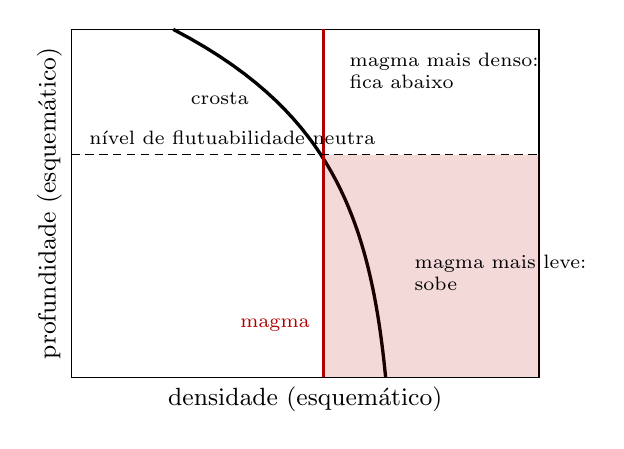
\begin{tikzpicture}[font=\scriptsize]
\begin{axis}[width=0.62\linewidth, height=6cm,
  xmin=0, xmax=1.15, ymin=0, ymax=1, y dir=reverse,
  xtick=\empty, ytick=\empty,
  xlabel={densidade (esquemático)}, ylabel={profundidade (esquemático)},
  label style={font=\small}, clip=false]
\addplot[very thick, black, domain=0:1, samples=40] ({0.25 + 0.55*(1 - exp(-3*x))}, {x});
\addplot[very thick, red!70!black] coordinates {(0.62,0) (0.62,1)};
\fill[red!70!black, opacity=0.15] (axis cs:0.62,0.36) rectangle (axis cs:1.15,1);
\draw[densely dashed] (axis cs:0,0.36) -- (axis cs:1.15,0.36);
\node[anchor=south west] at (axis cs:0.02,0.36) {nível de flutuabilidade neutra};
\node[anchor=east, black] at (axis cs:0.46,0.20) {crosta};
\node[anchor=east, red!70!black] at (axis cs:0.61,0.85) {magma};
\node[anchor=west, align=left] at (axis cs:0.82,0.70) {magma mais leve:\\sobe};
\node[anchor=west, align=left] at (axis cs:0.66,0.12) {magma mais denso:\\fica abaixo};
\end{axis}
\end{tikzpicture}
\par\smallskip{\small O \omterm{def:b2:magma-emplacement:ascent}{nível de flutuabilidade neutra} (esquemático). A densidade da
crosta aumenta com a profundidade, pela compactação dos sedimentos e pela passagem a
rochas mais densas; um \omterm{def:b2:magma-emplacement:magma}{magma} de densidade fixa sobe enquanto é mais leve que suas
encaixantes (sombreado) e se espalha onde as duas densidades se igualam.}
\end{omfigure}

Um \omterm{def:b2:magma-emplacement:bodies}{plúton} precisa abrir espaço para si. Ele pode levantar seu teto, como faz um \omterm{def:b2:magma-emplacement:bodies}{lacólito};
pode empurrar suas paredes para os lados onde elas são moles; pode preencher o espaço aberto por
falhamento; e pode desmoronar seu teto, bloco por bloco. Os grandes \omterm{def:b2:magma-emplacement:bodies}{plútons} foram por muito tempo
imaginados como enormes tanques de \omterm{def:b2:magma-emplacement:magma}{magma} alojados de uma só vez. A datação mudou essa
imagem. Os zircões da Suíte Intrusiva de Tuolumne, um \omterm{def:b2:magma-emplacement:bodies}{batólito} granítico na
Califórnia, mostram que ela foi alojada entre \num{95} e \qty{85}{Ma}, mais antiga
nas margens e mais jovem no centro, e uma de suas unidades sozinha ao longo de mais
de \qty{3}{Myr}, entre \qty{92.8}{Ma} e \qty{88.8}{Ma}. Um único corpo de
\omterm{def:b2:magma-emplacement:magma}{magma} de \qty{5}{km} de espessura e \qty{20}{km} de largura alojado a \qty{15}{km} de profundidade teria
se resfriado abaixo de \qty{750}{\celsius}, temperatura em que está cerca de meio cristalizado, em
cerca de \num{500000}~anos. Tais \omterm{def:b2:magma-emplacement:bodies}{plútons} devem ter sido montados incrementalmente,
a partir de muitas intrusões menores, como lâminas e \omterm{def:b2:magma-emplacement:bodies}{diques}, ao longo de milhões de anos
(\cref{exo:b2:magma-emplacement:11}).
% ledger: glazner04:tuolumne

\begin{omfigure}
\centering
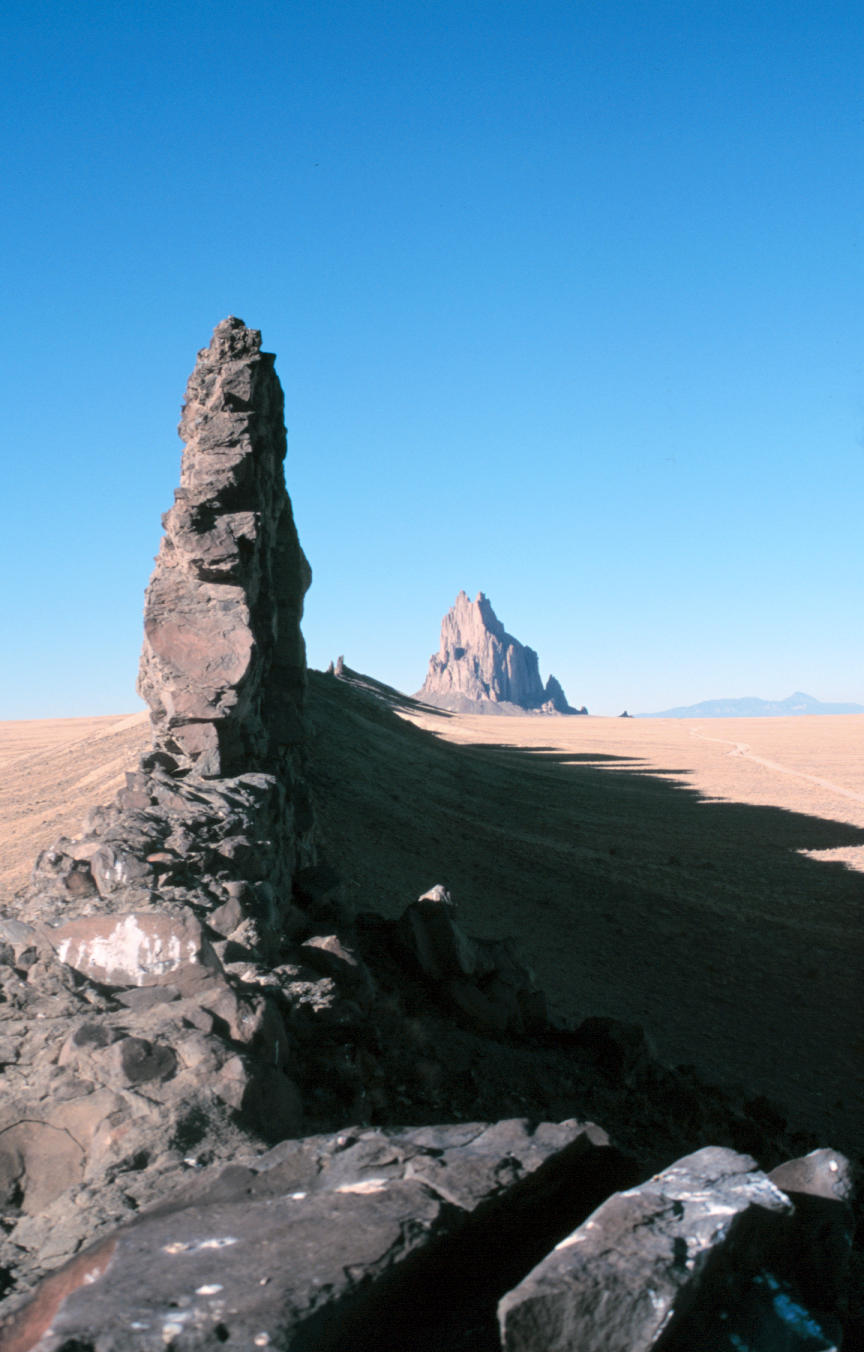
\includegraphics[width=0.3\linewidth]{images/book4/b2-shiprock-dyke.jpg}
\par\smallskip{\small Um \omterm{def:b2:magma-emplacement:bodies}{dique} perto de Shiprock, no Campo Vulcânico Navajo
(Novo México): a rocha do \omterm{def:b2:magma-emplacement:bodies}{dique} resistiu à erosão melhor que o arenito e o folhelho
que cortou, e hoje se ergue como um muro; ao fundo, o neck vulcânico do qual
irradiam vários \omterm{def:b2:magma-emplacement:bodies}{diques} como este. Fotografia: Dexter Perkins (CC0).}
\end{omfigure}

\section{Resfriamento e metamorfismo de contato}

Uma intrusão perde seu calor por condução para suas rochas encaixantes. O modelo mais
simples trata a intrusão e sua encaixante como um único meio condutor de
difusividade uniforme $\kappa$: no instante zero, uma lâmina de espessura $b$ está à temperatura
de intrusão $T_m$ e a encaixante a $T_0$. A solução da equação do calor, com
$x$ medido a partir do meio da lâmina, é
\[
T(x,t) = T_0 + \frac{T_m - T_0}{2}\left[\operatorname{erf}\frac{b/2 - x}{2\sqrt{\kappa t}}
+ \operatorname{erf}\frac{b/2 + x}{2\sqrt{\kappa t}}\right].
\]
A figura abaixo a mostra para uma \omterm{def:b2:magma-emplacement:bodies}{soleira} de \qty{100}{m} de espessura.
% ledger: delaney86b4:properties

\begin{proposition}[Temperatura de contato]\label{prop:b2:magma-emplacement:contact}
Nesse modelo, enquanto $\sqrt{\kappa t}$ é pequeno comparado com $b$, a
temperatura no contato da intrusão permanece na média $(T_m + T_0)/2$ das
temperaturas da intrusão e da encaixante.
\end{proposition}

\begin{proof}
No contato $x = b/2$, a primeira função erro é $\operatorname{erf}0 = 0$ e
a segunda é $\operatorname{erf}(b/(2\sqrt{\kappa t}))$, próxima de $1$ enquanto
$b \gg 2\sqrt{\kappa t}$. Então $T = T_0 + (T_m - T_0)/2$.
\end{proof}

Um \omterm{def:b2:magma-emplacement:bodies}{dique} basáltico a \qty{1150}{\celsius} em rochas a \qty{50}{\celsius} aquece assim
seu contato a \qty{600}{\celsius}. O calor de cristalização, tipicamente de
\qtyrange{700}{1000}{MJ/m^3}, mantém o \omterm{def:b2:magma-emplacement:magma}{magma} quente por mais tempo e eleva esse valor:
com \qty{900}{MJ/m^3} liberados entre \num{1150} e \qty{950}{\celsius}, o mesmo
modelo dá \qty{690}{\celsius}, enquanto condutividades dependentes da temperatura e encaixantes
úmidas reduzem as duas estimativas em 50 a \qty{75}{\celsius}.
% ledger: delaney86b4:dike, delaney86b4:properties

\begin{omfigure}
\centering
\begin{tikzpicture}
\begin{axis}[omrecord, width=0.86\linewidth, height=6cm,
  xmin=-200, xmax=200, ymin=0, ymax=1200,
  xlabel={distância ao meio da soleira (\unit{m})},
  ylabel={temperatura (\unit{\celsius})},
  legend pos=north east, legend style={font=\scriptsize},
  tick label style={font=\scriptsize}, label style={font=\small}]
\fill[gray!15] (axis cs:-50,0) rectangle (axis cs:50,1200);
\addplot[very thick, red!80!black] table[x=x_m, y=t1] {figdata/out/bachelor-2-magma-sill.dat};
\addlegendentry{1 ano}
\addplot[very thick, orange!90!black] table[x=x_m, y=t2] {figdata/out/bachelor-2-magma-sill.dat};
\addlegendentry{10 anos}
\addplot[very thick, blue!60!black] table[x=x_m, y=t3] {figdata/out/bachelor-2-magma-sill.dat};
\addlegendentry{50 anos}
\addplot[very thick, black] table[x=x_m, y=t4] {figdata/out/bachelor-2-magma-sill.dat};
\addlegendentry{200 anos}
\draw[densely dashed, gray] (axis cs:-200,625) -- (axis cs:200,625);
\node[font=\scriptsize, gray!40!black, anchor=south west] at (axis cs:-198,625) {$(T_m + T_0)/2$};
\node[font=\scriptsize, anchor=south] at (axis cs:0,20) {soleira};
\end{axis}
\end{tikzpicture}
\par\smallskip{\small Resfriamento por condução de uma \omterm{def:b2:magma-emplacement:bodies}{soleira} de \qty{100}{m} de espessura (sombreada),
intrudida a \qty{1150}{\celsius} em rocha a \qty{100}{\celsius}, com
$\kappa = \qty{0.7e-6}{m^2/s}$ e sem calor latente. O contato permanece perto de
\qty{625}{\celsius} durante décadas enquanto o calor se espalha na encaixante; após dois
séculos, a \omterm{def:b2:magma-emplacement:bodies}{soleira} e suas vizinhanças formam uma única zona morna e larga.}
\end{omfigure}
% ledger: delaney86b4:properties

A escala de tempo do resfriamento é o tempo de que o calor precisa para se difundir através da
intrusão, da ordem de $(b/2)^2/\kappa$: cerca de \num{16} dias para um \omterm{def:b2:magma-emplacement:bodies}{dique}
de \qty{2}{m} de largura, um século para uma \omterm{def:b2:magma-emplacement:bodies}{soleira} de \qty{100}{m} de espessura, cem mil anos
para um \omterm{def:b2:magma-emplacement:bodies}{plúton} de alguns quilômetros. O calor latente a alonga, assim como a
necessidade de solidificar o \omterm{def:b2:magma-emplacement:magma}{magma}, e não apenas resfriá-lo.

\begin{proposition}[Solidificação de uma intrusão]\label{prop:b2:magma-emplacement:stefan}
Suponha-se que um \omterm{def:b2:magma-emplacement:magma}{magma} à sua temperatura de solidificação $T_m$, com calor latente $L$ por unidade
de volume, ocupe o semiespaço $y > 0$ ao lado de uma rocha encaixante a $T_0$ que ocupa $y < 0$, ambos
de capacidade térmica $\rho c$ por unidade de volume e difusividade $\kappa$. A
frente de solidificação avança como $y_s = 2\lambda\sqrt{\kappa t}$, onde $\lambda$
é a raiz de
\[
\frac{L\sqrt\pi}{\rho c\,(T_m - T_0)} = \frac{e^{-\lambda^2}}{\lambda\,(1 + \operatorname{erf}\lambda)},
\]
e o contato permanece a $T_0 + (T_m - T_0)/(1 + \operatorname{erf}\lambda)$. Uma \omterm{def:b2:magma-emplacement:bodies}{soleira}
de espessura $b$, que se solidifica a partir das duas paredes, está sólida após
$t = b^2/(16\lambda^2\kappa)$.
\end{proposition}

\begin{proof}
O \omterm{def:b2:magma-emplacement:magma}{magma} à frente da frente permanece a $T_m$, de modo que o calor só flui no sólido
e na encaixante, onde se tenta $T = T_0 + (T_m - T_0)(1 + \operatorname{erf}\xi)/(1 +
\operatorname{erf}\lambda)$ com $\xi = y/(2\sqrt{\kappa t})$. Toda função de $\xi$
da forma $\alpha + \beta\operatorname{erf}\xi$ resolve a equação do calor; esta
tende a $T_0$ longe, dentro da encaixante ($\xi \to -\infty$), e é igual a $T_m$ na frente
$\xi = \lambda$. Em $y = 0$ ela dá a temperatura de contato enunciada. Na frente,
o calor latente liberado pelo sólido que avança, $L\,dy_s/dt = L\lambda\sqrt{\kappa/t}$
por unidade de área e de tempo, precisa ser conduzido para longe, $k\,\partial T/\partial y = k(T_m -
T_0)\,e^{-\lambda^2}/[(1 + \operatorname{erf}\lambda)\sqrt{\pi\kappa t}]$. Igualar os
dois e usar $k = \rho c\kappa$ dá a equação para $\lambda$. Cada parede da
\omterm{def:b2:magma-emplacement:bodies}{soleira} faz crescer sua própria frente, de modo independente enquanto o núcleo permanece a $T_m$; as duas
frentes se encontram quando $2\lambda\sqrt{\kappa t} = b/2$.
\end{proof}

Com o calor latente de um basalto e uma encaixante a cerca de \qty{100}{\celsius},
$\lambda$ vale cerca de $0.65$: uma \omterm{def:b2:magma-emplacement:bodies}{soleira} de \qty{100}{m} de espessura se solidifica em cerca de
setenta anos, e seu contato permanece perto de \qty{740}{\celsius} em vez de
\qty{625}{\celsius} durante esse tempo. O problema de fim de semana percorre esse caso.
Como o tempo cresce com o quadrado da espessura, uma \omterm{def:b2:magma-emplacement:bodies}{soleira} dez vezes mais espessa
leva cem vezes mais tempo.

\begin{definition}[Auréola de contato e suas rochas]\label{def:b2:magma-emplacement:aureole}
Uma \emph{margem resfriada}\index{margem resfriada} é a borda de granulação fina ou vítrea de uma
intrusão, onde o \omterm{def:b2:magma-emplacement:magma}{magma} se resfriou depressa contra uma encaixante mais fria. Uma
\emph{auréola de contato}\index{auréola de contato} é a zona de rocha encaixante em torno de uma
intrusão que foi metamorfizada por seu calor. O \emph{hornfels}\index{hornfels} é a
rocha dura, de granulação fina e não foliada em que se transformam os lamitos e as rochas vulcânicas em
uma auréola de contato. O \emph{escarnito}\index{escarnito} é a rocha formada onde fluidos
magmáticos quentes reagem com uma encaixante carbonática, depositando silicatos de cálcio, ferro e
magnésio, como granada e piroxênio, muitas vezes com magnetita e sulfetos metálicos.
\end{definition}
% ledger: earle:intrusive-bodies, earle:skarn

As \omterm{def:b2:magma-emplacement:aureole}{auréolas de contato} vão de alguns centímetros em torno de pequenos \omterm{def:b2:magma-emplacement:bodies}{diques} e \omterm{def:b2:magma-emplacement:bodies}{soleiras} a
várias dezenas de metros em torno de um grande stock, e o metamorfismo de contato abrange
de cerca de \qty{300}{\celsius} a mais de \qty{800}{\celsius}. Um lamito torna-se um
\omterm{def:b2:magma-emplacement:aureole}{hornfels}, um calcário um mármore, um arenito um quartzito. Um \omterm{def:b2:magma-emplacement:magma}{magma} alojado em profundidade
em rochas já quentes quase não produz auréola: a largura depende do
tamanho e da temperatura da intrusão e da temperatura de sua encaixante, como
prevê o modelo de resfriamento (\cref{exo:b2:magma-emplacement:12}). Os minerais que crescem em uma auréola,
e o que eles dizem sobre a temperatura, pertencem ao \cref{ch:b2:metamorphic-facies};
os metais que os \omterm{def:b2:magma-emplacement:aureole}{escarnitos} concentram, ao \cref{ch:b2:ore-deposits}.
% ledger: earle:skarn

\begin{inthefield}[Ler os contatos de um dique]
\begin{minipage}[t]{0.6\linewidth}\vspace{0pt}
Onde um \omterm{def:b2:magma-emplacement:bodies}{dique} aflora, um geólogo segue primeiro seus contatos com a rocha
encaixante. Uma margem de granulação mais fina ou mais vítrea que o centro do \omterm{def:b2:magma-emplacement:bodies}{dique} mostra
que o \omterm{def:b2:magma-emplacement:magma}{magma} foi resfriado bruscamente contra rocha fria; um \omterm{def:b2:magma-emplacement:bodies}{dique} de \qty{25}{cm} de largura estudado
na costa da Colúmbia Britânica tem margens resfriadas de \qty{2}{cm} de espessura. A rocha
encaixante é examinada junto ao contato em busca de cozimento: uma mudança de cor, um endurecimento,
minerais novos que desaparecem à medida que se afasta do \omterm{def:b2:magma-emplacement:bodies}{dique}. A largura da zona cozida e da
\omterm{def:b2:magma-emplacement:aureole}{margem resfriada}, comparada com a largura do \omterm{def:b2:magma-emplacement:bodies}{dique}, indica quão quente
estava a encaixante quando o \omterm{def:b2:magma-emplacement:bodies}{dique} chegou; um \omterm{def:b2:magma-emplacement:bodies}{dique} sem \omterm{def:b2:magma-emplacement:aureole}{margem resfriada} e sem
auréola foi intrudido em rochas que já estavam quentes. Coletam-se amostras através
do \omterm{def:b2:magma-emplacement:bodies}{dique}, da margem ao centro, para a geoquímica de seu fundido e para o
tamanho de seus cristais.
\end{minipage}\hfill
\begin{minipage}[t]{0.36\linewidth}\vspace{0pt}
\centering
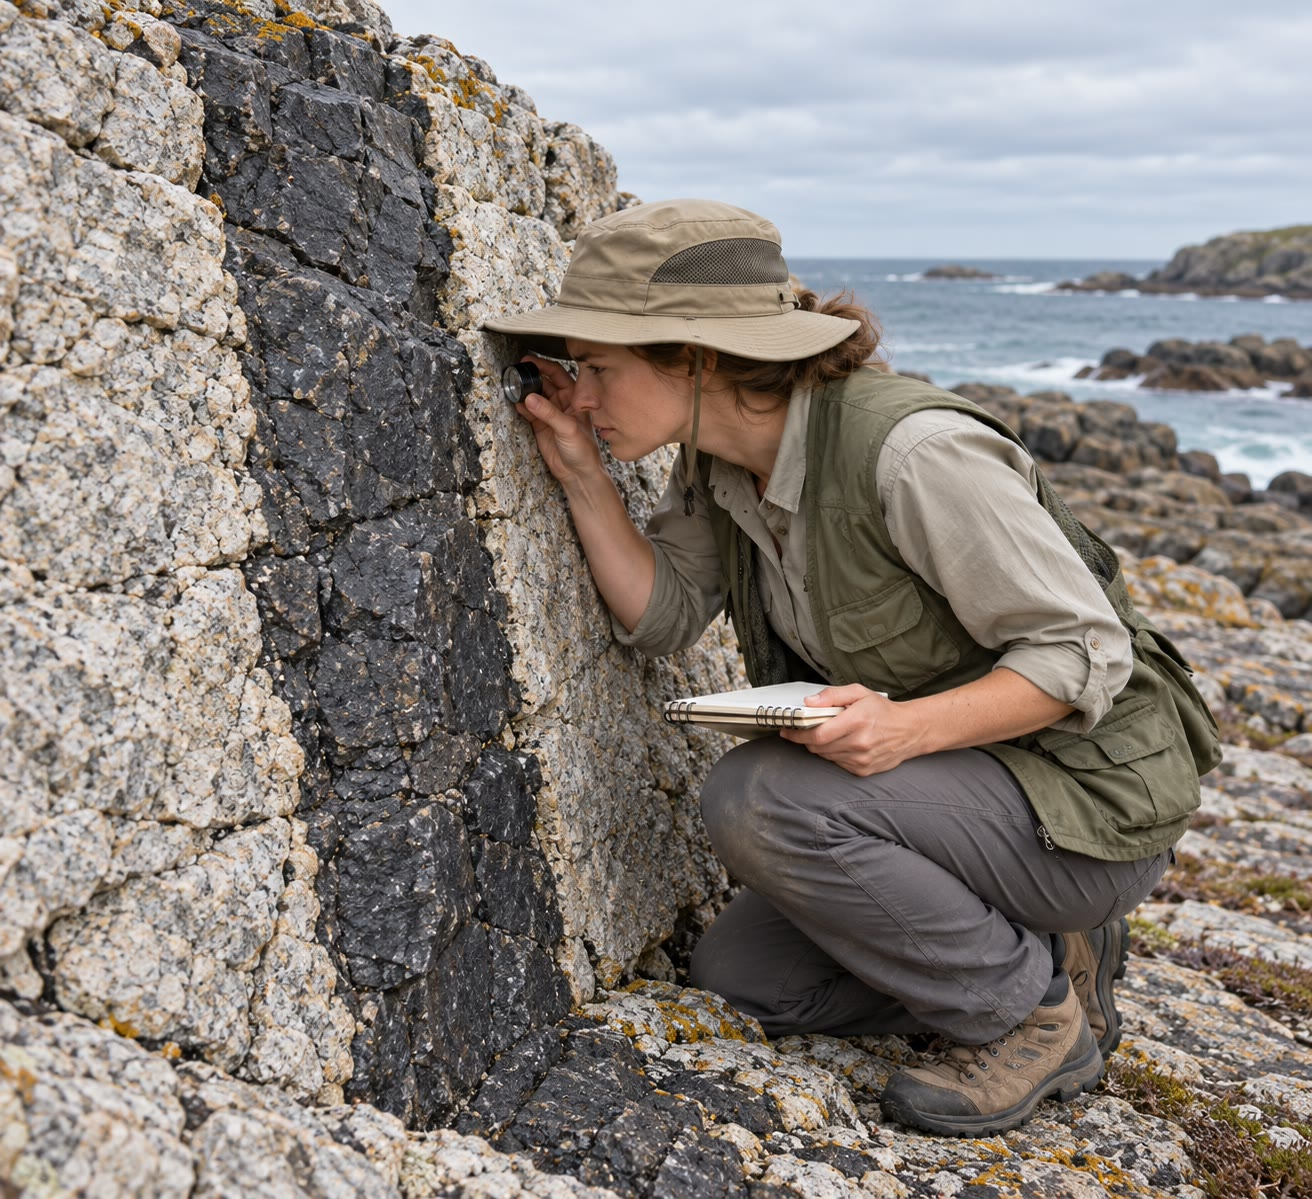
\includegraphics[width=\linewidth]{images/book4/ai/b2-dyke-contact.jpg}
\par\smallskip{\scriptsize Uma geóloga examina o contato de um \omterm{def:b2:magma-emplacement:bodies}{dique} escuro com uma
rocha encaixante clara (ilustração gerada por IA).}
\end{minipage}
\end{inthefield}
% ledger: earle:intrusive-bodies

\section{Exercícios}

\begin{exercise}[$\star$]\label{exo:b2:magma-emplacement:1}
Para fundidos graníticos hidratados, uma equação ajustada às medidas dá
$\log_{10}\eta = [-3.545 + 0.833\ln w] + [9601 - 2368\ln w]/\{T - [195.7 + 32.25\ln
w]\}$, com $\eta$ em \unit{Pa.s}, $w$ o teor de água em porcentagem em peso e $T$
em kelvins. Calcule $\log_{10}\eta$ a \qty{800}{\celsius} para $w = 1$ e $w = 4$,
e o fator pelo qual os três por cento adicionais de água reduzem a viscosidade.
\end{exercise}
% ledger: hd96:model

\begin{exercise}[$\star$]\label{exo:b2:magma-emplacement:2}
Com a lei da raiz quadrada, $s = 0.44$ para um riolito e $s = 0.34$ para um basalto
(por cento em peso por $\sqrt{\unit{MPa}}$), calcule a pressão de saturação de um
riolito com \qty{6}{\percent} de água e de um basalto com \qty{0.5}{\percent},
e as profundidades correspondentes em uma crosta de densidade \qty{2600}{kg/m^3}
($g = \qty{9.81}{m/s^2}$).
\end{exercise}

\begin{exercise}[$\star$]\label{exo:b2:magma-emplacement:3}
Calcule a temperatura de contato de um \omterm{def:b2:magma-emplacement:bodies}{dique} basáltico a \qty{1150}{\celsius}
intrudido em rochas a \qty{50}{\celsius}, depois em rochas a
\qty{400}{\celsius}. Qual dos dois \omterm{def:b2:magma-emplacement:bodies}{diques} terá a \omterm{def:b2:magma-emplacement:aureole}{margem resfriada} mais larga?
\end{exercise}

\begin{exercise}[$\star$]\label{exo:b2:magma-emplacement:4}
Dê o nome de cada corpo. (a) Uma lâmina de dolerito de \qty{30}{m} de espessura situada entre duas camadas
de arenito ao longo de \qty{20}{km}. (b) Uma lâmina vertical de basalto de \qty{2}{m} de largura
que corta calcários horizontais. (c) Um granito exposto em \qty{2000}{km^2},
formado por uma dúzia de unidades de idades diferentes. (d) Uma lente de pórfiro de \qty{1}{km} de diâmetro,
plana na base, acima da qual as camadas estão arqueadas. (e) Uma lâmina horizontal
de basalto em um granito.
\end{exercise}

\begin{exercise}[$\star\star$]\label{exo:b2:magma-emplacement:5}
Um fundido basáltico tem $\eta_{\ell} = \qty{100}{Pa.s}$. Com a relação de Einstein--Roscoe
($R = 1.35$), calcule a viscosidade do \omterm{def:b2:magma-emplacement:magma}{magma} com
\qty{5}{\percent}, \qty{20}{\percent}, \qty{40}{\percent} e \qty{60}{\percent} de
cristais, e compare o primeiro valor com a fórmula diluída de Einstein. Em que fração de cristais
a relação prevê o travamento?
\end{exercise}

\begin{exercise}[$\star\star$]\label{exo:b2:magma-emplacement:6}
Um \omterm{def:b2:magma-emplacement:magma}{magma} com densidade \qty{300}{kg/m^3} menor que a de suas paredes sobe por um \omterm{def:b2:magma-emplacement:bodies}{dique}.
(a) Para um basalto ($\eta = \qty{100}{Pa.s}$, $\rho = \qty{2700}{kg/m^3}$) em um \omterm{def:b2:magma-emplacement:bodies}{dique}
de \qty{1}{m} de largura, calcule a velocidade média, o fluxo por metro de \omterm{def:b2:magma-emplacement:bodies}{dique}, o
número de Reynolds e o tempo para subir \qty{10}{km}. (b) O mesmo tempo para um riolito de
\qty{e6}{Pa.s} em um \omterm{def:b2:magma-emplacement:bodies}{dique} de \qty{1}{m} de largura, depois de \qty{10}{m} de largura. (c) Um \omterm{def:b2:magma-emplacement:bodies}{dique}
de \qty{1}{m} de largura perde seu calor em um tempo da ordem de $(w/2)^2/\kappa$, com $\kappa =
\qty{1e-6}{m^2/s}$: qual das três ascensões pode ter êxito?
\end{exercise}

\begin{exercise}[$\star\star$]\label{exo:b2:magma-emplacement:7}
Um \omterm{def:b2:magma-emplacement:magma}{magma} de densidade \qty{2400}{kg/m^3} a \qty{900}{\celsius} libera
\qty{1}{\percent} de sua massa como vapor de água. Tratando o vapor como gás ideal
($R = \qty{8.314}{J/(mol.K)}$, \qty{18.015}{g/mol}), calcule a fração volumétrica de
gás no \omterm{def:b2:magma-emplacement:magma}{magma} a \qty{100}{MPa}, \qty{10}{MPa} e \qty{0.1}{MPa}. Qual dos
três valores é o menos confiável, e por quê?
\end{exercise}

\begin{exercise}[$\star\star$]\label{exo:b2:magma-emplacement:8}
Em uma bacia, a densidade das rochas aumenta com a profundidade $z$ como $\rho(z) =
2300 + 60\,z$ (\unit{kg/m^3}, $z$ em \unit{km}) até \qty{10}{km}. (a) Onde está
o \omterm{def:b2:magma-emplacement:ascent}{nível de flutuabilidade neutra} de um fundido basáltico de \qty{2650}{kg/m^3}? (b) O
modelo de densidade deste capítulo mostra que um por cento de água dissolvida reduz
a densidade de um fundido basáltico em cerca de \qty{70}{kg/m^3}. Onde para um fundido com
um por cento a mais de água? (c) Qual é a força de empuxo por metro cúbico
do fundido seco \qty{2}{km} abaixo de seu \omterm{def:b2:magma-emplacement:ascent}{nível de flutuabilidade neutra}?
\end{exercise}

\begin{exercise}[$\star\star$]\label{exo:b2:magma-emplacement:9}
Suponha que um \omterm{def:b2:magma-emplacement:ascent}{diápiro} granítico de raio \qty{1}{km} e déficit de densidade
\qty{300}{kg/m^3} suba através de uma crosta inferior de viscosidade \qty{e19}{Pa.s}. Calcule
sua velocidade de Stokes (esfera rígida) em milímetros por ano e o tempo para subir
\qty{10}{km}. Compare com a escala de tempo $a^2/\kappa$ de seu resfriamento, com $\kappa
= \qty{1e-6}{m^2/s}$. O que você conclui?
\end{exercise}

\begin{exercise}[$\star\star\star$]\label{exo:b2:magma-emplacement:10}
A água se dissolve em um fundido ao mesmo tempo como moléculas, $x_m = K_1 f$, e como grupos
hidroxila, $x_{\mathrm{OH}}^2 = K_2 x_m$ (com o oxigênio do fundido em grande excesso), de modo
que a água dissolvida total é $x = x_m + x_{\mathrm{OH}}/2$. (a) Exprima $x$ em
função de $f$ e mostre que ele se comporta como $\sqrt f$ para $f$ baixo e como $f$ para
$f$ alto. (b) Em que fugacidade as duas formas de água são igualmente abundantes? (c)
Com $K_1 = \qty{1e-4}{MPa^{-1}}$ e $K_2 = 0.2$, calcule essa fugacidade e a
fração de água dissolvida como hidroxila a \qty{100}{MPa}.
\end{exercise}

\begin{exercise}[$\star\star\star$]\label{exo:b2:magma-emplacement:11}
Um \omterm{def:b2:magma-emplacement:bodies}{plúton} granítico de \qty{1000}{km^3} é montado ao longo de \qty{4}{Myr}. (a) Calcule
seu suprimento médio de \omterm{def:b2:magma-emplacement:magma}{magma} em \unit{km^3} por ano e em \unit{m^3} por segundo. (b) Um
único \omterm{def:b2:magma-emplacement:bodies}{dique} de \qty{1}{km} de comprimento e \qty{2}{m} de largura, com velocidade média de
\qty{0.8}{m/s}, o alimenta: quanto tempo o \omterm{def:b2:magma-emplacement:bodies}{dique} levaria para fornecer todo o
\omterm{def:b2:magma-emplacement:bodies}{plúton}? Que fração dos \qty{4}{Myr} isso representa? (c) Se o \omterm{def:b2:magma-emplacement:bodies}{plúton} é formado por
lâminas de \qty{20}{m} de espessura e \qty{10}{km} por \qty{10}{km} de extensão, quantas lâminas
são necessárias, e quanto tempo separa duas delas em média? (d) Com
$\lambda = 0.65$ e $\kappa = \qty{0.7e-6}{m^2/s}$, quanto tempo uma lâmina leva para se
solidificar? O \omterm{def:b2:magma-emplacement:bodies}{plúton} chega a ser um único grande corpo de \omterm{def:b2:magma-emplacement:magma}{magma}?
\end{exercise}

\begin{exercise}[$\star\star\star$]\label{exo:b2:magma-emplacement:12}
Longe de um \omterm{def:b2:magma-emplacement:bodies}{dique} delgado de largura $b$ (a distâncias $x \gg b$), seu calor age como uma
fonte plana instantânea: $T - T_0 = (T_m - T_0)\,b\,e^{-x^2/(4\kappa
t)}/\sqrt{4\pi\kappa t}$. (a) Mostre que, à distância $x$, a temperatura é máxima em
$t^* = x^2/(2\kappa)$, e que essa elevação máxima é $\Delta T_{\max} = (T_m -
T_0)\,b/(x\sqrt{2\pi e})$. (b) Para um \omterm{def:b2:magma-emplacement:bodies}{dique} de \qty{2}{m} de largura com $T_m - T_0 =
\qty{1100}{K}$, a que distância a rocha se aquece no máximo \qty{100}{K}, e
quando ($\kappa = \qty{0.7e-6}{m^2/s}$)? (c) Por que as auréolas dos \omterm{def:b2:magma-emplacement:bodies}{diques} delgados são tão
estreitas?
\end{exercise}

\section{Problema: a soleira sob o planalto}

\begin{problem}[{Problema de fim de semana --- seguir um magma basáltico de seu dique
alimentador até uma soleira, sua água e o tempo que a soleira leva para se solidificar}]
\label{pb:b2:magma-emplacement:1}
Sob um planalto imaginário, sedimentos (folhelho e arenito) de densidade média
\qty{2450}{kg/m^3} repousam a \qty{3.0}{km} de profundidade sobre um embasamento cristalino de
densidade \qty{2800}{kg/m^3}. Um \omterm{def:b2:magma-emplacement:magma}{magma} basáltico subiu de \qty{15}{km} por um \omterm{def:b2:magma-emplacement:bodies}{dique}
de \qty{2.0}{m} de largura e se espalhou ao longo da base dos sedimentos como uma \omterm{def:b2:magma-emplacement:bodies}{soleira} de dolerito
de \qty{100}{m} de espessura. Dados: temperatura de intrusão \qty{1150}{\celsius}; lei de
viscosidade do fundido $\log_{10}\eta = -4.55 + 5510/(T - 611)$ ($T$ em kelvins); densidade
do fundido com sua água \qty{2710}{kg/m^3}; \qty{20}{\percent} de cristais em volume
(Einstein--Roscoe, $R = 1.35$); água dissolvida \qty{0.40}{\percent}, solubilidade
$s = 0.34$ por cento por $\sqrt{\unit{MPa}}$; temperatura da encaixante no nível da \omterm{def:b2:magma-emplacement:bodies}{soleira}
\qty{100}{\celsius}; $\kappa = \qty{0.7e-6}{m^2/s}$, $\rho c = \qty{2.5}{MJ/(m^3.K)}$,
calor latente \qty{900}{MJ/m^3}, sendo o \omterm{def:b2:magma-emplacement:magma}{magma} tratado como se solidificando à sua
temperatura de intrusão; $g = \qty{9.81}{m/s^2}$; um ano vale \qty{3.156e7}{s}.

\medskip\noindent\textbf{Parte I --- O magma.}
\begin{enumerate}
\item Calcule $\log_{10}\eta$ e $\eta$ do fundido a \qty{1150}{\celsius}
(\qty{1423}{K}).
\item O mesmo a \qty{1100}{\celsius}. Por que fator a viscosidade varia nesses
\qty{50}{K}?
\item Calcule a viscosidade do \omterm{def:b2:magma-emplacement:magma}{magma} com seus cristais a
\qty{1150}{\celsius}.
\item Em que fração de cristais a relação de Einstein--Roscoe faria o
\omterm{def:b2:magma-emplacement:magma}{magma} travar? Compare com a estimativa de campo do fim do escoamento em massa.
\item Calcule a diferença de densidade entre o \omterm{def:b2:magma-emplacement:magma}{magma} e o embasamento, e
entre o \omterm{def:b2:magma-emplacement:magma}{magma} e os sedimentos.
\item Calcule a pressão litostática no nível da \omterm{def:b2:magma-emplacement:bodies}{soleira}.
\end{enumerate}

\noindent\textbf{Parte II --- Subindo pelo dique.}
\begin{enumerate}[resume]
\item Calcule o gradiente de pressão de empuxo $\Delta\rho\,g$ que impele o \omterm{def:b2:magma-emplacement:magma}{magma}
através do embasamento.
\item Calcule a velocidade média do \omterm{def:b2:magma-emplacement:magma}{magma} no \omterm{def:b2:magma-emplacement:bodies}{dique}.
\item Calcule o fluxo por metro de \omterm{def:b2:magma-emplacement:bodies}{dique}, e o fluxo total se o \omterm{def:b2:magma-emplacement:bodies}{dique} tiver
\qty{1.0}{km} de comprimento.
\item Calcule o número de Reynolds do escoamento. Ele é laminar?
\item Quanto tempo o \omterm{def:b2:magma-emplacement:magma}{magma} leva para subir de \qty{15}{km} a \qty{3.0}{km}?
\item Compare com a escala de tempo $(w/2)^2/\kappa$ em que o \omterm{def:b2:magma-emplacement:bodies}{dique} perde seu
calor. Ele consegue permanecer aberto?
\item Explique por que o \omterm{def:b2:magma-emplacement:magma}{magma} parou a \qty{3.0}{km} e se espalhou lateralmente, usando
o vocabulário do capítulo.
\end{enumerate}

\noindent\textbf{Parte III --- A água.}
\begin{enumerate}[resume]
\item Calcule a pressão de saturação da água do fundido, e a profundidade nos
sedimentos em que ela é atingida.
\item Quanta água o fundido poderia conter no nível da \omterm{def:b2:magma-emplacement:bodies}{soleira}? O \omterm{def:b2:magma-emplacement:magma}{magma} da \omterm{def:b2:magma-emplacement:bodies}{soleira}
exsolve água?
\item As vesículas da \omterm{def:b2:magma-emplacement:aureole}{margem resfriada} da \omterm{def:b2:magma-emplacement:bodies}{soleira} contêm sobretudo CO$_2$. Explique.
\item Se todos os \qty{0.40}{\percent} de água saíssem na superfície, a
\qty{1150}{\celsius} e \qty{0.1}{MPa}, que fração volumétrica do \omterm{def:b2:magma-emplacement:magma}{magma}
o vapor ocuparia (gás ideal)?
\end{enumerate}

\noindent\textbf{Parte IV --- Resfriamento e solidificação.}
\begin{enumerate}[resume]
\item Desprezando o calor latente, calcule a temperatura de contato da \omterm{def:b2:magma-emplacement:bodies}{soleira}.
\item Desprezando o calor latente, calcule a temperatura \qty{10}{m} acima do contato
superior \num{10}~anos após a intrusão.
\item Mesmo modelo: calcule a temperatura no meio da \omterm{def:b2:magma-emplacement:bodies}{soleira} após
\num{10}~anos e \num{50}~anos.
\item Mesmo modelo: \qty{80}{m} acima do contato superior, calcule a temperatura após
\num{300}, \num{363} e \num{420} anos. A rocha ali chega a atingir
\qty{300}{\celsius}?
\item Calcule $L\sqrt\pi/(\rho c\,(T_m - T_0))$ para a \omterm{def:b2:magma-emplacement:bodies}{soleira}.
\item Calcule $e^{-\lambda^2}/(\lambda(1 + \operatorname{erf}\lambda))$ para $\lambda = 0.64$,
$0.65$ e $0.66$ ($\operatorname{erf}0.64 = 0.6346$, $\operatorname{erf}0.65 = 0.6420$,
$\operatorname{erf}0.66 = 0.6494$), e dê $\lambda$ com duas casas decimais.
\item Com calor latente, calcule a temperatura de contato enquanto a \omterm{def:b2:magma-emplacement:bodies}{soleira}
se solidifica. Por que ela é mais alta que na questão 18?
\item Calcule a escala de tempo $(b/2)^2/\kappa$ em anos.
\item Calcule o tempo que a \omterm{def:b2:magma-emplacement:bodies}{soleira} leva para se solidificar, em anos, o número-chave deste
problema, e explique por que ele é mais curto que a escala de tempo da questão
anterior, embora o calor latente precise ser removido.
\end{enumerate}
\end{problem}
% ledger: grd08:model, kolz22:einstein-roscoe, glazner04:tuolumne, moore98:h2o, lowenstern01:co2, delaney86b4:properties
